\documentclass[11pt,a4paper]{article}

\usepackage[top=1.25in,left=1.0in,right=1.0in,footskip=0.5in]{geometry}
\usepackage[usenames,dvipsnames]{xcolor}
\usepackage[slovene,english]{babel}
\usepackage[utf8]{inputenc}
\usepackage{fancyhdr}
\usepackage{graphicx}
\usepackage{hyperref}
\usepackage{listings}
\usepackage{siunitx} 
\usepackage{subfig}

\DeclareGraphicsExtensions{.pdf,.eps,.png,.jpg}
\hypersetup{colorlinks=true, linkcolor=LimeGreen, citecolor=LimeGreen, urlcolor=cyan}
\lstset{basicstyle=\scriptsize, frame=single, tabsize=12, title=Example file {\bf\lstname}}

\pagestyle{fancy}
\fancyhf{}
\lhead{\footnotesize\bf Introduction to Network Analysis ({\color{magenta}INA})}
\rhead{\footnotesize\bf Homework {\color{magenta}\#2}}
\cfoot{\thepage}
\fancypagestyle{titlestyle}{
\rhead{\footnotesize\bf Spring 2020/21}
\cfoot{}}

\definecolor{titc}{RGB}{106,40,134}
\definecolor{dfnc}{RGB}{155,187,90}
\definecolor{dfac}{RGB}{80,131,189}

\newcommand{\dfn}[1]{{\it\color{dfnc}#1}}
\newcommand{\dfa}[1]{{\color{cyan}#1}}
\newcommand{\hid}[1]{{\color{gray}#1}}
\newcommand{\cmp}[1]{\mathcal{O}(#1)}
\newcommand{\prb}[1]{\mathrm{P}(#1)}
\newcommand{\avg}[1]{\langle#1\rangle}

\newcommand{\hint}[1]{{\it (#1)}}
\newcommand{\point}{({\color{magenta}$1$~point})}
\newcommand{\points}[1]{({\color{magenta}$#1$~points})}
\newcommand{\total}{({\color{magenta}1 point})}
\newcommand{\totals}[1]{({\color{magenta}#1 points})}
\newcommand{\figref}[1]{{\color{LimeGreen}Figure~\ref{fig:#1}}}
\newcommand{\tblref}[1]{{\color{LimeGreen}Table~\ref{tbl:#1}}}

\newcommand{\gnm}{$G(n,m)$\xspace}
\newcommand{\gnp}{$G(n,p)$\xspace}
\newcommand{\gk}{$G(\{k\})$\xspace}

\setcounter{page}{0}

\begin{document} 

\thispagestyle{titlestyle}

\vspace*{0.05in} 
\begin{center} 
	{\huge\bf Homework {\color{magenta}\#2}} 
\end{center} 
\vspace*{0.05in} 

\paragraph{} This homework is complete and will not be changed. The homework does not require a lot of writing, but may require some thinking. It does not require a lot of processing power, but may require efficient programming. It accounts for $13.3\%$ of the course grade. Any questions and comments regarding the homework should be directed to \href{https://piazza.com/class/kkn1oz577n2sq}{Piazza}.

\section*{Submission details}

\paragraph{} This homework is due on {\bf\color{magenta} April 9th} at 9:00pm, while late days expire on {\bf\color{magenta} April 12th} at 12:00pm. The homework must be submitted through (1) \href{https://www.gradescope.com}{Gradescope} (entry code {\bf NM8ZRM}) and (2) \href{https://ucilnica.fri.uni-lj.si/course/view.php?id=183}{eUcilnica}. (1)~Submission to \href{https://www.gradescope.com}{Gradescope} should include answers to all questions, each on a separate page, which may also demand pseudocode, proofs, tables, plots, diagrams and other. (2)~Submission to \href{https://ucilnica.fri.uni-lj.si/course/view.php?id=183}{eUcilnica} should include at least this cover sheet with signed honor code and all the programming code used to complete the exercises. The homework is considered submitted only when \textit{both} parts have been submitted. Failing to include this honor code in the submission will result in {\bf\color{LimeGreen} 10\% deduction}. Failing to submit all the developed code will result in {\bf\color{LimeGreen} 50\% deduction}.

\section*{Honor code}

\paragraph{} Students are strongly encouraged to discuss the homework with other classmates and form study groups. Yet, each student must then solve the homework by her/himself without the help of others and should be able to redo the homework at a later time. In other words, students are encouraged to collaborate, but should not copy from one another. Referring to any solutions obtained from classmates, course books, previous years, found online or other material, is considered an honor code violation. Also, stating any part of the solutions in class or on \href{https://piazza.com/class/kkn1oz577n2sq}{Piazza} is considered an honor code violation. Finally, failing to name the correct study group members, or filling out the wrong date or time of the submission, is also considered an honor code violation. Honor code violation will not be tolerated! Any student violating the honor code will be reported to {\bf\color{LimeGreen} faculty disciplinary committee} and vice dean for education.

\vspace*{0.15in}
\paragraph{Name \& SID:} \rule{4.5in}{0.5pt}
\paragraph{Study group:} \rule{4.5in}{0.5pt}
\paragraph{Date \& time:} \rule{2.5in}{0.5pt}
\paragraph{} I acknowledge and accept the honor code.
\paragraph{Signature:} \rule{2.5in}{0.5pt}

\pagebreak

\section{Where is SN100? \totals{0.75}}

\paragraph{} \figref{dolphins} shows social network of \href{http://lovro.lpt.fri.uni-lj.si/ina/nets/dolphins}{bottlenose dolphins} famously studied by Lusseau~\cite{LSBHSD03}. After the disappearance of a particular dolphin named SN100 during the course of experiment~\cite{LN04}, the rest split into two groups shown with different colors in~\figref{clusters}. Your task is to analyze whether network analysis could be utilized to detect this obviously important role of SN100. 

\begin{figure}[h] \centering
	\subfloat[Division into {\bf two groups}]{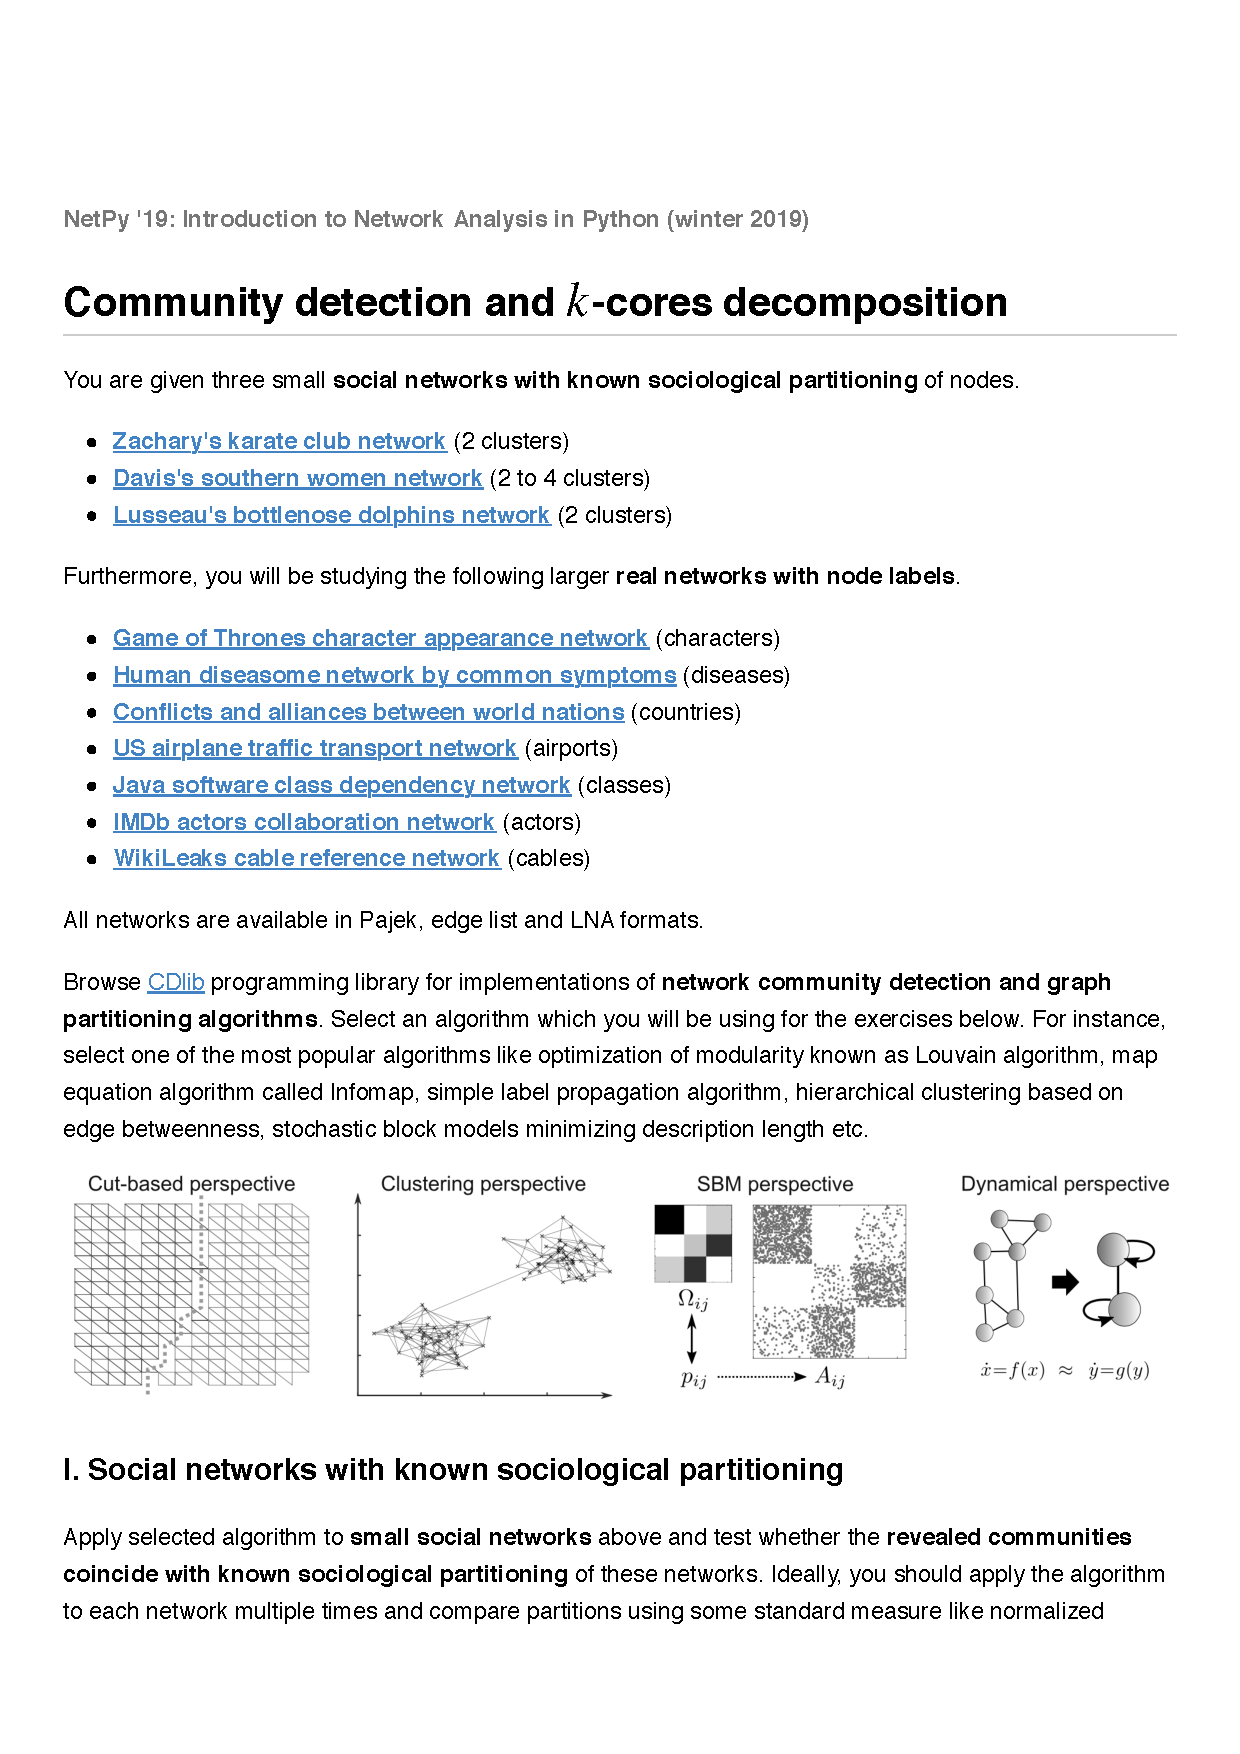
\includegraphics[width=0.4\textwidth]{clusters}\label{fig:clusters}}
	\subfloat[{\bf Betweenness centrality}]{
\includegraphics[width=0.4\textwidth]{betweenness}\label{fig:betweenness}}
	\caption{{\bf Lusseau bottlenose dolphins network}}
	\label{fig:dolphins}
\end{figure}

\paragraph{} You can use any network analysis method, algorithm or technique. State how you measured the importance of SN100 and provide all necessary results.

\subsection*{What to submit?}

\paragraph{} State how you measured the importance of SN100 and briefly discuss the results \points{2\times 0.25}. Give a printout of all the code used to solve the exercise \points{0.25}.

\section{Is software scale-free? \totals{2}}

\paragraph{} Consider two software class dependency networks~\cite{SB11b} representing \href{http://lovro.lpt.fri.uni-lj.si/ina/nets/java}{Java language} and \href{http://lovro.lpt.fri.uni-lj.si/ina/nets/lucene}{Lucene search engine} (\figref{lucene}). These are directed networks where node $i$ links to node $j$ if software class represented by $i$ depends on or {\it uses} class represented by $j$. Compute degree distributions $p_k$ of both networks and plot each $p_k$ on a separate log-log plot by representing each distinct $(k,p_k)$ with a single dot, $k>0$. \hint{Transformation to logarithmic axes should be done by your plotting software.} Next, compute also in-degree distributions $p_{k^{in}}$ and out-degree distributions $p_{k^{out}}$ of both networks, and superimpose them on the same plots using dots of different color. 

\begin{figure}[h] \centering
	\subfloat[Colors show {\bf node in-degree}]{\includegraphics[width=0.4325\textwidth]{indegree}}
	\subfloat[Colors show {\bf node out-degree}]{\includegraphics[width=0.4325\textwidth]{outdegree}}
	\caption{{\bf Lucene class dependency network}}
	\label{fig:lucene}
\end{figure}

\paragraph{} Compare all three degree distributions $p_{k^{\cdot}}$ of each network and highlight the differences among them. Do the distributions appear to be scale-free following a power-law $k_{\cdot}^{-\gamma_{\cdot}}$? For the distributions not appearing like a power-law, reason why. For the distributions that seem to follow a power-law, reason why and compute their power-law exponent $\gamma_{\cdot}$ using maximum likelihood formula~\cite{Bar16}
$$\gamma_{\cdot}=1+n_{\cdot}\left[\sum_{i=1}^{n}\ln\frac{k_i^{\cdot}}{k_{min}^{\cdot}-\frac{1}{2}}\delta(k_i^{\cdot}\geq k_{min}^{\cdot})\right]^{-1},$$
where $k_i^{\cdot}$ is $\cdot$-degree of node $i$, $k_{min}^{\cdot}\geq 1$ is some reasonable choice for the minimum degree cutoff and $n_{\cdot}\leq n$ is the number of nodes thus considered.

\subsection*{What to submit?}

\paragraph{} Draw two plots with three distributions each and briefly discuss the results \points{3\times 0.25}. Reason whether distributions are scale-free and why, and compute $\gamma_{\cdot}$ and $k^{\cdot}_{min}$ of seemingly scale-free distributions \points{4\times 0.25}. Give a printout of all the code used to solve the exercise \points{0.25}.

\section{Errors and attacks on the Internet \totals{2}}

\paragraph{} Consider \href{http://lovro.lpt.fri.uni-lj.si/ina/nets/nec}{Internet overlay map} represented by an undirected graph. Routers, switches and hubs on the Internet fail from time to time. Your task is to study how this affects the Internet's ability to stay connected. Simulate such failure by random removal of nodes and measure the fraction of nodes in the largest connected component in the resulting network. Next, consider also a malicious individual attacking the Internet. Simulate such attack by removing most highly linked nodes or hubs and again measure the fraction of nodes in the largest connected component. For each of the two scenarios, plot the fraction of nodes in the largest connected component after removing $0\%$, $10\%$, $20\%$, $30\%$, $40\%$ and $50\%$ of randomly selected nodes or hubs. Finally, repeat the experiments also for a random graph~\cite{ER59} with the same number of nodes and links as the Internet map. 

\paragraph{} Briefly discuss the results by comparing robustness of the Internet and random graph. Would you claim that the Internet is robust to random failures? Would you claim that the Internet is robust to malicious attacks? What about random graphs? Can you explain your reasoning by some structural property of the Internet and/or random graphs.

\subsection*{What to submit?}

\paragraph{} Draw two plots showing the robustness of the Internet and random graph \points{3\times 0.25}. Briefly comment on the results and give answers to all four questions \points{4\times 0.25}. Give a printout of all the code used to solve the exercise \points{0.25}.

\section{HIV and network sampling \totals{1.75}}

\paragraph{} When a patient is diagnosed with HIV, in most Western countries, she/he will be questioned about past sexual contacts. The authorities would then make an effort to track down those contacts and test them for HIV. The process is repeated with anyone who also tests positive, tracing her/his contacts as well, until all leads have been exhausted. This process is called contact tracing. 

\paragraph{} Notice that contact tracing gives a (biased) sample of the underlying social network~\cite{LF06}. Assuming that one gets HIV from a random sexual contact, contact tracing can be approximated by simple random walk. Simulate a random walk on  small \href{http://lovro.lpt.fri.uni-lj.si/ina/nets/social}{social network} until you sample $10\%$ of the nodes and take {\it induced} graph on the sampled nodes for your sampled network. 

\paragraph{} Is the original social network small-world~\cite{WS98} and/or seemingly scale-free~\cite{BA99}? Is the sampled network small-world and/or seemingly scale-free? Can you reason why? Support your answers with necessary computations. 

\subsection*{What to submit?}

\paragraph{} Give brief answers to all three questions and provide necessary results to support your reasoning \points{3\times 0.5}. Give a printout of all the code used to solve the exercise \points{0.25}.

\section{Who to vaccinate? \totals{0.5}}

\paragraph{} Probability that an individual would spread the disease through her/his social network is proportional to $k^2$~\cite{New10}, where $k$ is the degree of corresponding node. Consider two immunization schemes for preventing the spread of diseases. In the first scheme, you randomly select some number of individuals and vaccinate them. In the second scheme, you select the same individuals, but then rather vaccinate a random acquaintance of theirs. 

\paragraph{} Which of the two schemes do you expect to provide better immunization? Why?

\subsection*{What to submit?}

\paragraph{} Give brief answers to both questions \points{2\times 0.25}.

\bibliographystyle{alpha}
\bibliography{../misc/bibliography}

\end{document}
